\begin{frame}{Analizador básico}
  \begin{block}{Objetivo}
    Desarrollar un módulo que capture el sonido del micrófono, lo analice y
    detecte la nota que se está tocando.
  \end{block}

\end{frame}

\begin{frame}{Analizador básico}
  \begin{center}
    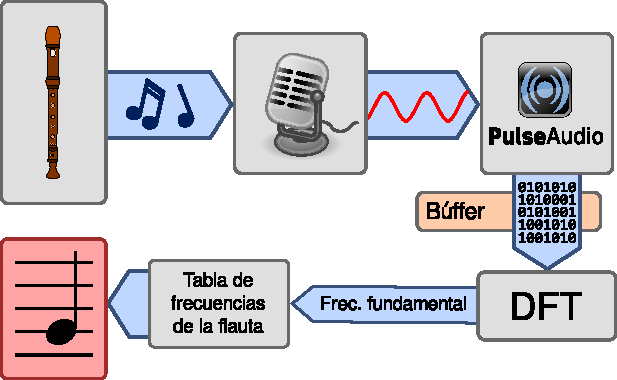
\includegraphics{imagenes/esquema_analizador}
  \end{center}
\end{frame}

\begin{frame}{Analizador básico}
  \begin{block}{Primer paso: capturar el audio}
    \begin{itemize}
    \item Se utilizó la API de PulseAudio.
    \item Abrimos un flujo de entrada.
    \item Creamos un búffer para recoger los datos.
    \item Procesamos los datos cuando se llena el búffer.
    \end{itemize}
    
  \end{block}
\end{frame}

\begin{frame}{Analizador básico}
  \begin{block}{Segundo paso: analizar el sonido}
    \begin{itemize}
    \item Trabajamos con el contenido del búffer.
    \item Aplicamos el algoritmo DFT.
    \item Aislamos la frecuencia fundamental.
    \item Comparamos la frecuencia fundamental con una tabla de frecuencias para
      la flauta dulce.
    \item Devolvemos la nota detectada.
    \end{itemize}
  \end{block}  
\end{frame}

\begin{frame}[fragile]{Carga de fuentes TrueType}
  \begin{center}
    oFlute utiliza \textbf{Gosu} como sistema gráfico.
    
    \begin{itemize}
    \item Open Source.
    \item Ofrece renderizado 2D con aceleración por hardware.
    \item Acceso a la entrada del usuario.
    \item Multiplataforma: Windows, Linux, Mac.
    \item API muy sencilla, orientada a objetos.
    \item Desarrollo ágil.
    \end{itemize}
  \end{center}
\end{frame}

\begin{frame}[fragile]{Carga de fuentes TrueType}
  \begin{center}
    \textcolor{red}{\textbf{Problema:}} Gosu no permite cargar fuentes TrueType
    en GNU/Linux.

    \pause
    \medskip
    
    \textcolor{dgreen}{\textbf{Solución:}} se implementa un módulo propio para
    carga y pintado de fuentes TrueType. \pause\\[1em]Este módulo se liberó y pasó a
    formar \textbf{parte oficial} de Gosu.
  \end{center}
  \begin{minted}{cpp}
// Used for custom TTF files
// Adapted from customFont class by Jose Tomas Tocino Garcia (TheOm3ga)
class SDLTTFRenderer : boost::noncopyable
  \end{minted}
\end{frame}

\begin{frame}{Animaciones dinámicas}
  \begin{center}
    \textcolor{red}{\textbf{Problema:}} uno de los objetivos era tener
    interfaces amigables, fluidas y minimalistas.

    \pause \medskip

    \textcolor{dgreen}{\textbf{Solución:}} se desarrolla un sistema de
    animaciones mediante interpolaciones de movimiento.

    \pause\medskip

    Permite movimientos de aceleración, deceleración, uniformes, etcétera. Es
    extensible a un número arbitrario de atributos.

    \pause\medskip

    Se basó en las ecuaciones de Robert Penner, \\liberadas bajo licencia BSD.
    
  \end{center}  
\end{frame}

\begin{frame}{Internacionalización}
  \begin{center}
    \textcolor{red}{\textbf{Problema:}} con miras a otros países, resultaría
    necesario internacionalizar el proyecto.

    \pause \medskip

    \textcolor{dgreen}{\textbf{Solución:}} \textbf{GNU Gettext} como sistema de
    internacionalización. 

    \medskip

    Es el sistema de i18n más popular, con multitud de herramientas y
    comunidades de traducción colaborativa, como Launchpad.
    
    \pause\medskip

    Su estudio derivó en la publicación del documento \textit{Traducción de
      proyectos con GNU gettext en 15 minutos}
    \footnote{\url{http://hdl.handle.net/10498/10772}}.

  \end{center}
\end{frame}
%%% Local Variables: 
%%% mode: latex
%%% TeX-master: "../presentacion"
%%% End: 
